\documentclass{beamer}
\usetheme{CambridgeUS}
\title{AI1110 Assignment I (ICSE Class 10 2017)}
\author{Narsupalli Sai Vamsi (cs21btech11038)}
\begin{document}
\maketitle
\textbf{Question 1c:} \\
AB and CD are two parallel chords of a circle such that 
AB = 24cm and CD = 10cm. if the radius of the circle is 13cm,
find the distance between the two chords.
\begin{figure}
    \centering
    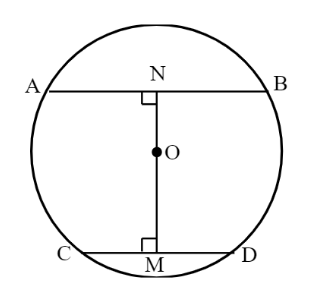
\includegraphics[width=\columnwidth]{./fig1.png}
    \caption{}
    \label{fig:1}
\end{figure} \\
\textbf{Solution} \\
Let us take O as origin \\
$\vec{OA}$ is position vector of A, $\vec{OB}$ is position vector of B,
$\vec{OC}$ is position vector of C, $\vec{OD}$ is position vector of D,
$\vec{ON}$ is position vector of N, $\vec{OM}$ is position vector of M,\\

The value we have to find is magnitude of \textbf{MN}.
By using the traingle law of vector addition i.e when two vectors are represented as two sides of the triangle with the order of magnitude and direction, then the third side of the triangle represents the magnitude and direction of the resultant vector.\\
we can say
\begin{align}
\vec{OA} = \vec{ON}+\vec{AN}\\
\vec{OB} = \vec{ON}+\vec{BN}\\
\vec{OC} = \vec{OM}+\vec{CM}\\
\vec{OD} = \vec{OM}+\vec{DM}\\
\vec{MN} = \vec{OM}-\vec{ON}
\end{align}
from one of the equations in 1st two , and from one of the other equations in last two we can find the magnitude of $\vec{ON}$,$\vec{OM}$\\
$\lvert \vec{ON} \rvert$ =$\lvert \vec{OA}-\vec{AN} \rvert$ \\
$\lvert \vec{OM} \rvert$ =$\lvert \vec{OC}-\vec{CM} \rvert$ \\
Given that the radius is 13cm \\
\implies $\lvert \vec{OA}\rvert$ , $\lvert \vec{OC} \rvert$ = 13cm\\
We know that perpendicular to a chord of a circle from centre bisects the chord into equal parts. \\
\implies $\lvert \vec{AN} \rvert$ = 12cm , $\lvert \vec{ON} \rvert = 5cm\\
\lvert \vec{ON} \rvert = \sqrt {{\lvert \vec{OA} \rvert}^2 - {\lvert \vec{AN} \rvert}^2} \\
\lvert \vec{ON} \rvert = \sqrt {{13}^2 - {12}^2} \\
\lvert \vec{ON} \rvert = \sqrt{25}\\
\lvert \vec{ON} \rvert = 5cm\\
\lvert \vec{OM} \rvert = \sqrt {{\lvert \vec{OC} \rvert}^2 - {\lvert \vec{CM} \rvert}^2} \\
\lvert \vec{OM} \rvert = \sqrt{{13}^2 - {5}^2}\\
\lvert \vec{OM} \rvert = \sqrt{144}\\
\lvert \vec{OM} \rvert = 12cm\\
From equation 0.5 we can say\\
$\lvert \vec{MN} \rvert =$\lvert \vec{OM}-\vec{ON} \rvert$ \\
from vector law of subtraction we get \\
$\lvert \vec{MN} \rvert =$\lvert \vec{OM}\rvert$ + $\lvert \vec{ON}\rvert$ \\
$\lvert \vec{MN} \rvert = 12 + 5 cm\\
\implies \lvert \vec{MN} \rvert = 17cm
\end{document}
